\chapter{Limitaciones y amenazas a la validez}
\label{chap:limitaciones}

Cada limitación se enuncia aquí junto a la cifra que permite dimensionarla: una salvedad que no
puede cuantificarse no dice cuánto hay que descontar de las conclusiones. La
Tabla~\ref{tab:limitaciones} las reúne ordenadas por severidad.

{\footnotesize
\input{tables/t08_limitaciones.tex}
}

\noindent\footnotesize{La severidad es un juicio del autor sobre cuánto condiciona cada limitación
las conclusiones, no una medida estadística.}\normalsize

Cuatro de esas filas merecen una precisión que la tabla no puede contener.

La \textbf{multiplicidad} se agravó dos veces y a propósito: al encadenar tres Model Studies y al
recorrer 1.440 carteras. Sus dos alcances no deben confundirse. La predictiva contamina la métrica
que el trabajo reporta como resultado principal; la de la rejilla no puede tocar el Rank-IC y se
limita a convertir el Information Ratio de la ventana de selección en una cota superior optimista.
Ninguna de las dos anula el contraste de permutación, que no depende del número de configuraciones
ensayadas.

El \textbf{predominio del agente de riesgo} queda matizado y agravado a la vez por su atribución
local. Matizado, porque ese agente no resulta ser una réplica de la prima de baja volatilidad y
reasigna atención entre sus variables según el régimen. Agravado, porque desplaza la incógnita sin
resolverla: el trabajo no explica \emph{por qué} unas variables de estructura de negociación a
semanas ordenan retornos a doce meses, y una señal cuyo mecanismo no se comprende es más frágil ante
un cambio de régimen que una respaldada por una hipótesis económica.

La \textbf{concentración en pocos nombres} no la delata ninguna métrica agregada: de las 42 acciones
que pasaron por la cartera, la primera aporta 27,8 puntos de contribución neta y las cinco primeras
suman algo más de la mitad de lo que aportan las quince mayores; en la era reservada una sola
posición aporta 21,3 de los puntos de la ventana. El número de apuestas realmente independientes es
por tanto bastante menor que los diez años de serie.

Y la que más condiciona las conclusiones: \textbf{el orden predictivo y el pago económico no se
mueven en la misma dirección}. El Rank-IC es mayor en la era más reciente, mientras que el
Information Ratio de la cartera por defecto cae y se vuelve negativo en esa misma era. La cartera
adoptada corrige ese deterioro ---no deja ningún año negativo en la ventana de selección---, pero
que hiciera falta cambiar la cartera para lograrlo es justamente la limitación: la consecuencia para
el alcance del trabajo es que la evidencia de que el modelo \emph{ordena} es más sólida que la de
que esa ordenación \emph{se cobra}.

\section{Amenazas a la validez interna}

\subsection{Fechas, restatements y calidad de la fuente}

El diseño point-in-time reduce de forma directa el \textit{lookahead bias}, pero depende de la
calidad de las fechas de filing y de la correspondencia entre métricas de Finnhub y periodos
contables. Los restatements históricos pueden ser invisibles en años tempranos: que una cifra esté
hoy disponible con una fecha de filing antigua no garantiza que sea idéntica a la cifra que conoció
el mercado ese día. La mitigación consiste en conservar periodo, filing y lag de ejecución, y en no
presentar la fuente como una cinta histórica perfecta.

\subsection{El sesgo de supervivencia por cobertura del proveedor}

La pertenencia histórica al índice limita el sesgo de supervivencia de composición, pero no elimina
la cobertura desigual de las empresas retiradas. A diferencia de la versión habitual de esta
salvedad, aquí no es una posibilidad genérica sino algo medido, y se sabe de ella tres cosas.

La \textbf{causa} está medida en el Capítulo~\ref{chap:datos} y no es la mortalidad empresarial sino
la retirada de símbolos por parte del proveedor de precios. El dato que remata el diagnóstico es
cómo crece la ausencia con el tiempo transcurrido desde que una empresa salió del índice.

\begin{figure}[htbp]
  \centering
  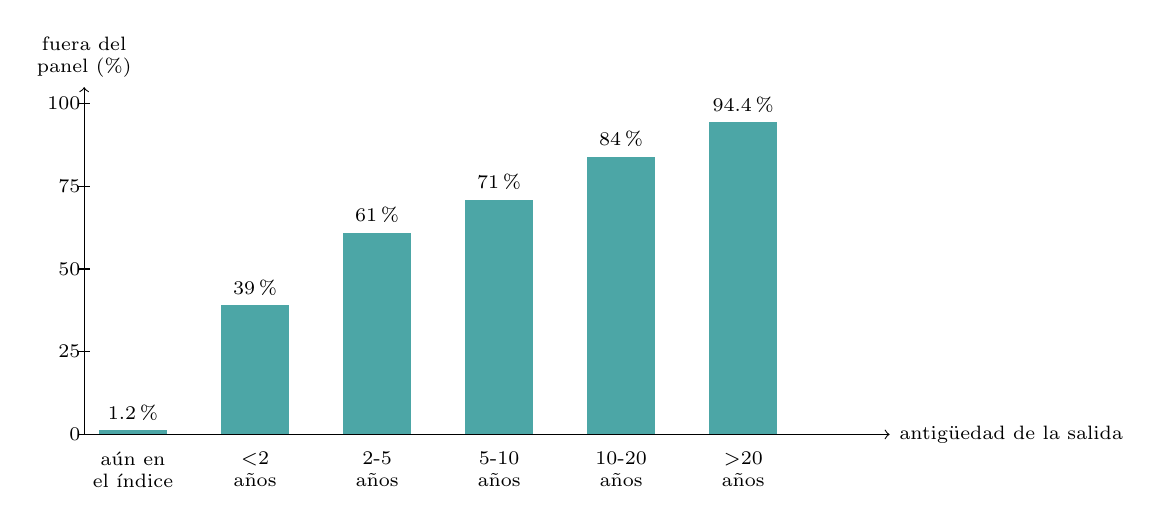
\begin{tikzpicture}[font=\footnotesize]
    \begin{scope}[x=1.55cm,y=0.042cm]
      \draw[->] (-0.4,0) -- (6.2,0) node[right,font=\scriptsize] {antigüedad de la salida};
      \draw[->] (-0.4,0) -- (-0.4,105) node[above,font=\scriptsize,align=center] {fuera del\\panel (\%)};
      \foreach \y in {0,25,50,75,100}
        {\draw (-0.45,\y)--(-0.35,\y) node[left,font=\scriptsize] {\y};}
      \foreach \x/\v/\l in {0/1.2/{aún en\\el índice}, 1/39/{$<$2\\años}, 2/61/{2-5\\años},
                            3/71/{5-10\\años}, 4/84/{10-20\\años}, 5/94.4/{$>$20\\años}}
        {\fill[teal!70] (\x-0.28,0) rectangle (\x+0.28,\v);
         \node[above,font=\scriptsize] at (\x,\v) {\v\,\%};
         \node[below=1mm,align=center,font=\scriptsize] at (\x,0) {\l};}
    \end{scope}
  \end{tikzpicture}
  \caption{Fracción de empresas que no llegan al panel, según cuánto hace que abandonaron el índice.
  La progresión es la firma de una fuente que poda su histórico, no la de un sector que quiebra.}
  \label{fig:ausencia-antiguedad}
\end{figure}

La Figura~\ref{fig:ausencia-antiguedad} lo muestra sin ambigüedad: entre las empresas que siguen hoy
en el índice falta el 1,2\,\%, mientras que entre las que salieron hace más de veinte años falta el
94,4\,\%. Si el problema fuera la mortalidad empresarial, la ausencia no dependería de la
antigüedad de esa manera.

La \textbf{dirección} es optimista, no conservadora. Las empresas que sí llegan al panel sobreviven
hasta hoy con mucha más frecuencia que los miembros reales del índice de su año: en 1998 lo hacen el
77,7\,\% frente al 35,5\,\%, un exceso de 42 puntos porcentuales que se reduce a cero en 2026. Como
el entrenamiento es una ventana móvil, el exceso que afecta a cada evaluación decae de 26,2 puntos
al evaluar 2015 a 8,0 al evaluar 2026.

Podría objetarse que, como muchas de las ausentes fueron adquiridas con prima, el sesgo sería
conservador. Ese razonamiento cuenta cabezas en vez de permanencia: una empresa adquirida rinde una
vez y desaparece, mientras que una superviviente compone durante todo el periodo, y es esa
composición la que infla el resultado.

Queda por declarar el \textbf{límite de lo demostrable}. Lo medido es la composición del universo,
no el retorno de las empresas ausentes, que carecen precisamente de la serie de precios que
permitiría calcularlo: el sesgo \emph{no se cuantifica en puntos de rentabilidad}. Un dato acota su
alcance en la dirección contraria ---los ausentes sí tienen fundamentales descargados, así que la
exclusión no selecciona empresas opacas sino símbolos sin precio---, y la lectura por eras es la
comprobación empírica de si mueve o no el resultado predictivo. Una réplica con una fuente comercial
\textit{point-in-time} sería la prueba definitiva.

\section{Amenazas económicas y de generalización}

Los costes son constantes, 10 pb de comisión y 20 pb de \textit{slippage}, y no modelan impacto de
mercado, \textit{bid--ask} dinámico ni fiscalidad. La sensibilidad medida acota esta limitación
mejor de lo que suele acotarse: el exceso de la cartera no se agota hasta unos \CosteEquilibrio{}
puntos básicos por operación, \MargenCoste{} veces el coste adoptado, de modo que el resultado no
depende de haber elegido una comisión benévola. Esa holgura, sin embargo, se calcula sobre la ventana
de selección, donde la cartera es la mejor de la rejilla. En la era reservada se reduce a
\CosteEquilibrioReservado{} puntos básicos con las decisiones congeladas y desaparece por completo al
resimular la cartera, porque allí el resultado empata con el índice: no hay margen que gastar en
fricción.

El universo estadounidense de gran capitalización limita además la extrapolación a pequeñas
empresas, otros países o regímenes de liquidez distintos.

Cada limitación acota una afirmación diferente, y conviene no mezclarlas: la multiplicidad limita el
Sharpe, el solapamiento limita la precisión, la cobertura limita la generalización y la cartera
limita la transferencia de señal. Ninguna permite ignorar los placebos, la permutación o la
estabilidad por eras.

\section{Lo que la cartera dejó de ganar}

Las limitaciones anteriores acotan lo que puede afirmarse del resultado medido. Hay otra que no
aparece en ninguna métrica agregada, porque no es un error sino el precio de una regla: cada vez que
la cartera vende una posición para comprar otra mejor, renuncia a lo que la vendida hiciera después.

El sistema registra esos casos. En la ventana de selección hubo quince ventas seguidas de una subida
apreciable en los doce meses posteriores, y la Tabla~\ref{tab:ventas-prematuras} recoge las ocho
mayores.

\begin{table}[htbp]
  \centering
  \small
  \caption{Ventas que el mercado desmintió: exceso no cobrado en los doce meses siguientes.}
  \label{tab:ventas-prematuras}
  \begin{tabular}{llrrr}
\toprule
Acción & Fecha de venta & Subida posterior & Índice & Exceso no cobrado \\
\midrule
BA & 2017-10-30 & 37,7\% & 6,2\% & 29,7\% \\
ROK & 2016-08-29 & 38,4\% & 14,4\% & 21,0\% \\
PH & 2016-09-29 & 43,7\% & 19,4\% & 20,4\% \\
AZO & 2017-10-30 & 26,6\% & 6,2\% & 19,3\% \\
APH & 2023-07-30 & 42,6\% & 20,3\% & 18,6\% \\
APTV & 2016-07-30 & 34,8\% & 16,0\% & 16,2\% \\
COST & 2018-10-30 & 32,9\% & 15,8\% & 14,7\% \\
VLO & 2016-07-30 & 33,0\% & 16,0\% & 14,6\% \\
\bottomrule
\end{tabular}

  \caption*{Todas se vendieron por el mismo motivo: otra candidata ofrecía mayor ventaja neta
  esperada.}
\end{table}

La mayor es Boeing, vendida en octubre de 2017: subió un 37,7\,\% en el año siguiente frente al
6,2\,\% del índice, de modo que la cartera dejó sobre la mesa casi treinta puntos de exceso. Las tres
siguientes rondan los veinte. En conjunto son quince episodios, no una anécdota, y todos comparten el
mismo motivo de venta: apareció una candidata con más ventaja neta esperada.

Hay una asimetría en cómo el trabajo cuenta su propio resultado que este dato ayuda a corregir. El
Capítulo~\ref{chap:resultados-economicos} dedica una sección a explicar por qué el sistema compró
Apple y la mantuvo cuarenta y cuatro meses, y esa es la cara favorable. La desfavorable es que las
posiciones que peor salieron ---la peor resta 4,2 puntos de contribución neta tras dieciocho meses en
cartera--- se mantuvieron también durante mucho tiempo, porque la misma permanencia mínima que
protege a las buenas protege a las malas.

Dos salvedades acotan lo que puede leerse aquí, y son importantes. La primera es que estos quince
casos se identifican \emph{con el resultado ya conocido}: sabemos que subieron porque miramos después.
No puede derivarse de ellos ninguna regla nueva, porque añadir un filtro que los hubiera evitado sería
ajustar sobre el resultado. La segunda es de selección: la tabla recoge las ventas que el mercado
desmintió, no las que acertó, y esas últimas no se listan en ninguna parte. Lo que la tabla mide es el
coste de la regla de rotación, no su balance neto.

\section{Limitaciones heredadas del desarrollo}

\subsection{Tres decisiones que condicionan las cifras}

Tres limitaciones no proceden del diseño sino de decisiones tomadas durante el desarrollo. Merecen
figurar aquí porque afectan a la interpretación de las cifras y no serían visibles para un lector
que sólo viera el resultado final; su origen y la disyuntiva técnica que las motivó se documentan en
el Anexo~\ref{anexo:desarrollo}.

La primera es la salvaguarda de la curva de alfa: una recta fija entre $-10$\,\% y $+10$\,\% que
sustituye a la calibración empírica cuando ninguna ventana de la cascada produce una pendiente
creciente. Su defecto no es de magnitud sino de dirección: es un supuesto \emph{a priori} que se
dispara \textbf{precisamente cuando la evidencia indica que no hay señal que calibrar}, de modo que
allí donde interviene la expectativa de alfa no procede de los datos sino de la recta declarada. El
diseño la prefiere a no tener alfa esperada en absoluto ---sin ella la cartera no podría decidir
umbrales en esos tramos---, pero hay que declararla como lo que es: una decisión de diseño
discutible, no una medición.

La segunda es que la calibración isotónica que precedió a esa salvaguarda se retiró sin conservarla
como opción del catálogo, de modo que este trabajo \emph{no puede} ofrecer una comparación empírica
entre ambas formulaciones; la afirmación de que la nueva es mejor descansa en un argumento sobre el
estimador, no en una medición pareada.

La tercera afectaba a las variables de cartera, que en versiones anteriores de este trabajo tomaban
su valor del catálogo recomendado y no de una medición, de modo que las cifras económicas debían
leerse como una cota inferior. El Portfolio Study resuelve esa limitación y la sustituye por otra de
naturaleza distinta: la cartera ya no es arbitraria, pero es la mejor de 1.440 evaluadas sobre la
ventana de selección, y por tanto sus cifras dentro de esa ventana son ahora una cota \emph{superior}
optimista en lugar de una inferior conservadora. La comprobación de la era reservada es la única
lectura de esas cifras que no está sujeta a ese sesgo, y descansa sobre poco más de un año de datos.

\subsection{Decisiones con margen escaso}

De las dieciocho decisiones de la pasada de referencia, dieciséis conservaron el valor heredado y
sólo dos lo cambiaron. Una de esas dos ---la variable de régimen de mercado--- ganó por no
inferioridad, es decir, sin demostrar ser mejor; la otra ---la tasa de aprendizaje--- sí dominó al
valor previo, pero con una ventaja media de tres diezmilésimas de Rank-IC y acertando en el
50,5\,\% de las cohortes emparejadas. Que la cadena apenas mueva al ganador indica convergencia y no
fragilidad, pero ninguno de esos dos valores puede presentarse como un hallazgo empírico: la
medición que los respalda no distingue con holgura entre las alternativas.
